\begin{frame}[hoved]
\frametitle{Vulnerability: Priority-Based Scheduling}

FreeRTOS uses a priority-based preemptive scheduler --- inherently unfair and vulnerable.

\vspace{0.3cm}
\begin{center}
\resizebox{0.70\textwidth}{!}{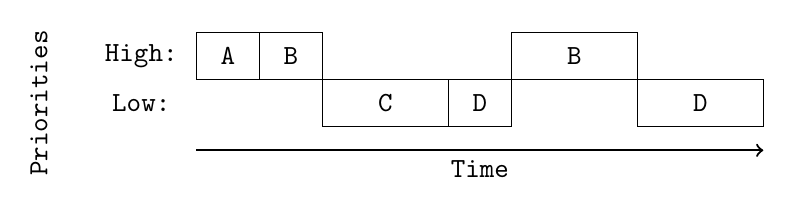
\begin{tikzpicture}[font=\ttfamily]

    % Style for general text nodes
    \tikzset{lbl/.style={inner sep=1pt, align=center}}

    % Define vertical coordinates for rows and labels
    \def\barheight{0.6} % Height of each bar
    \def\vtopprio{1.5}   % Vertical center of the top bar row
    \def\vsecprio{\vtopprio - \barheight} % Vertical center of the CM' bar row
    \def\ytimeline{\vsecprio - \barheight} % Vertical position of the minor frames timeline

    % Define standard tick positions
    \def\timeslice{0.8}

    % --- Bar Rows (drawn inside outlines) ---

    % Row 1: Top prio
    \draw (0, \vtopprio-\barheight/2) rectangle (\timeslice, \vtopprio+\barheight/2) 
      node[lbl, midway]{A};
    \draw (\timeslice, \vtopprio-\barheight/2) rectangle (\timeslice*2, \vtopprio+\barheight/2)
      node[lbl, midway]{B};

    % Row 2: Second prio
    \draw (\timeslice * 2, \vsecprio-\barheight/2) rectangle (\timeslice * 4, \vsecprio+\barheight/2)
      node[lbl, midway]{C};
    \draw (\timeslice * 4, \vsecprio-\barheight/2) rectangle (\timeslice*5, \vsecprio+\barheight/2)
      node[lbl, midway]{D};

    \draw (\timeslice*5, \vtopprio-\barheight/2) rectangle (\timeslice*7, \vtopprio+\barheight/2)
      node[lbl, midway]{B};

    \draw (\timeslice * 7, \vsecprio-\barheight/2) rectangle (\timeslice*9, \vsecprio+\barheight/2)
      node[lbl, midway]{D};

    % --- Left Vertical Label ---
    \node[lbl, rotate=90] at (-2.0, {\vsecprio}) {Priorities};
    \node[lbl] at (-0.7, {\vtopprio}) {High:};
    \node[lbl] at (-0.7, {\vsecprio}) {Low:};

    % Timeline axis with arrow and label
    \draw[thick, ->]
        (0, \ytimeline)
        -- node[below] {Time}
        (9*\timeslice, \ytimeline);
\end{tikzpicture}

}
\end{center}

\vspace{0.3cm}
\textbf{The channel:} A high-priority task signals \texttt{0} or \texttt{1} by sleeping or running, and the low-priority task measures its own wake time.

\end{frame}

\begin{frame}[hoved]
\frametitle{Design: Domain Scheduling}

\textbf{Chosen approach:} Domain-level scheduling

\vspace{0.1cm}
\begin{columns}[T,onlytextwidth]
\begin{column}{0.48\textwidth}
\centering
\scriptsize Static domains\\[0.05cm]
\resizebox{0.8\textwidth}{!}{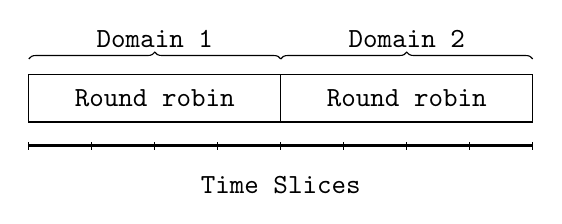
\begin{tikzpicture}[font=\ttfamily]

    % Style for general text nodes
    \tikzset{lbl/.style={inner sep=1pt, align=center}}

    % Define vertical coordinates for rows and labels
    \def\barheight{0.6} % Height of each bar
    \def\vtopprio{1.5}   % Vertical center of the top bar row
    \def\ytimeline{\vtopprio - \barheight} % Vertical position of the minor frames timeline

    % Define standard tick positions
    \def\timeslice{0.8}

    % --- Bar Rows (drawn inside outlines) ---

    % First domain
    \path[draw, decorate, decoration=brace] (0, \vtopprio + 0.5) -- (\timeslice * 4, \vtopprio + 0.5) node[lbl, midway, above, yshift=0.3em]{Domain 1};
    \draw (0, \vtopprio-\barheight/2) rectangle (\timeslice*4, \vtopprio+\barheight/2) 
      node[lbl, midway]{Round robin};

    % Second domain
    \path[draw, decorate, decoration=brace] (\timeslice * 4, \vtopprio + 0.5) -- (\timeslice * 8, \vtopprio + 0.5) node[lbl, midway, above, yshift=0.3em]{Domain 2};
    \draw (\timeslice*4, \vtopprio-\barheight/2) rectangle (\timeslice*8, \vtopprio+\barheight/2) 
      node[lbl, midway]{Round robin};

    % Main timeline axis
    \draw[thick] (0, \ytimeline) -- (8*\timeslice, \ytimeline);

    % Intermediate ticks (not all but to give structure)
    \foreach \x in {0, ..., 8} {
         \draw (\x*\timeslice, \ytimeline-0.05) -- (\x*\timeslice, \ytimeline+0.05);
    }

    % Central label below the timeline
    \node[lbl] at ( { 4 * \timeslice }, \ytimeline-0.5 ) {Time Slices};

\end{tikzpicture}

}
\end{column}
\hfill
\begin{column}{0.48\textwidth}
\centering
\scriptsize Dynamic domains\\[0.05cm]
\resizebox{0.8\textwidth}{!}{\input{figures/dynamic_domain_sched.tex}}
\end{column}
\end{columns}

\vspace{0.2cm}
\begin{itemize}
  \item Domains receive fixed time slices
  \item Tasks within a domain use standard priority scheduling
  \item Time protection is enforced only \textit{between} domains
\end{itemize}

\end{frame}
